\documentclass[conference]{IEEEtran}
\usepackage{cite}
\usepackage{amsmath,amssymb,amsfonts}
\usepackage{algorithmic}
\usepackage{graphicx}
\usepackage{textcomp}
\usepackage{xcolor}
\usepackage[normalem]{ulem}
\usepackage[english]{babel}
\def\BibTeX{{
	\rm B\kern-.05em{\sc i\kern-.025em b}\kern-.08em
	T\kern-.1667em\lower.7ex\hbox{E}\kern-.125emX
}}
\renewcommand{\arraystretch}{1.3}

\begin{document}
\title{
	The Great Processor Shortage:\\
	History and Projection of an Emerging Trend
}

\author{
	\IEEEauthorblockN{1\textsuperscript{st} Dang Vo}
	\IEEEauthorblockA{
		\textit{Faculty of IT} \\
		\textit{University of Science}\\
		Ho Chi Minh, Vietnam \\
		vndang21@vp.fitus.edu.vn
	}
	\and
	\IEEEauthorblockN{2\textsuperscript{nd} Hau Nguyen}
	\IEEEauthorblockA{
		\textit{Faculty of IT} \\
		\textit{University of Science}\\
		Ho Chi Minh, Vietnam \\
		ntthau21@vp.fitus.edu.vn
	}
	\and
	\IEEEauthorblockN{3\textsuperscript{rd} Vinh Thai}
	\IEEEauthorblockA{
		\textit{Faculty of IT} \\
		\textit{University of Science}\\
		Ho Chi Minh, Vietnam \\
		tvvinh21@vp.fitus.edu.vn
	}
	\and
	\IEEEauthorblockN{4\textsuperscript{th} Thuc Doan}
	\IEEEauthorblockA{
		\textit{Faculty of IT} \\
		\textit{University of Science}\\
		Ho Chi Minh, Vietnam \\
		dnthuc21@vp.fitus.edu.vn
	}
}

\maketitle

\begin{abstract}
	% Todo Write and Revise
\end{abstract}

\begin{IEEEkeywords}
	CPU, Correlation, Economics, Electronics\\
	industry, GPU, Polynomial regression, Semiconductor shortage.
\end{IEEEkeywords}

\section{Introduction}
Imagine it's the simpler times of around the start of 2019. You, a
hard-working corporate employee, haven't a care in the world about your
dusty old desktop as your company already provides you with high-end ones
at work. As 2020 hits, so does the COVID-19 pandemic, and now you must
work from home. Fast forward to 2021, you have just gotten accustomed to
remote working on your sub-par desktop. And then disaster strikes, your
graphics card fails on you. At first, you are utterly enraged. But then,
you start to sympathize with your 7-year-old card: ``Maybe it's time for
an upgrade'' -- you thought. You start scouring the internet for a
replacement only to be hard-pressed to find that the average graphics
card price has skyrocketed from \$267 to a whopping \$1077 in just under 2
years \cite{Dave:2022}!

But how did all this happen? Indeed, The COVID-19 pandemic has been a
great detriment to our societies for almost half a decade. It has not
only disrupted our daily lives but also advancements in various
fields. One such field is the field of processing unit development, i.e.,
the field concerning the development of CPUs and GPUs. Coupled with the
pandemic, over the past few years, this field has been relentlessly attacked
by various advents such as the China-United States trade war, cryptocurrency
mining, the Russia-Ukraine war...\cite{Wikipedia:2023} to the point of
stagnation. At the supply's
end, due to the shutdown of virtually all supply lines of intermediate
products, processor manufacturers have been struggling to acquire enough
materials to keep up with the rising demands. While at the demand's end,
long periods of lockdowns imply a surge in remote work creating an
increase in demand for computers in which processors reside. These
factors caused prices to shoot up to unprecedented figures which led to
the great processor shortage in the second half of 2020.

The processor shortage has caused great disruptions in various
industries, largely those who utilize processors in their production
procedures. However, though mostly detrimental, the shortage gave rise to
many significant innovations in processor architectures in order to
reduce the manufacturing cost, thus lowering the barrier of entry to
processors. Naturally, two questions arise: First, when will the
shortage, along with all its demerits, subside and end? And second, how
will the processor industry change from the shortage? But the insight
into the future lies within the past and thus, we must first take a step
back into the past and investigate the history of the great
processor shortage. Hence the title (and purpose) of the research.

Although there have been a few efforts in tackling the impact of the
computer chip shortage, as stated in section \ref{RelatedWorks}, these
efforts are made mostly to address the shortcomings of the computer chip
supply chains rather than the actual developments of the chip itself.
Furthermore, there does not appear to be any rigorous attempt at predicting
when the shortage will end. All in all, to the
best of our knowledge, an investigation into when the shortage will end and how
it will impact the development of processors has not yet been \textbf{formally}
studied.

Answering these questions will provide us with an insight into why the
shortage happened and how to prevent such a catastrophe in the future.
Furthermore, knowledge of when the shortage ends will tell us if the
shortage is long-term or short-term. This will aid manufacturers to be
more flexible in timely adjusting the level of production to suit the
ever-changing demands. All in all, the research will help get the state
of the economy back on track and ensure its stability for the near future.

The research will leverage datasets on common metrics of processors to
analyze the evolution of both the processor shortage and the processors
themselves during the pandemic using statistics. Armed with that knowledge,
the paper will attempt to project when the shortage ends and what is the
next big trend for the processor industry. To achieve this, we will employ
the help of a polynomial regression model -- A reliable tool for short-term
predictions. By feeding it historical data, it can learn the hidden
patterns and be able to predict the future of the development of
processing units.

It can be said that there are many factors which contribute to the
processor shortage. However, the research will only
address the impact of past advents on the great processing unit
shortage and not potential future events. Moreover, the research will only
dissect in detail the trend in
performance, efficiency, and value in CPUs and GPUs from the first quarter of
2017 to the first quarter of 2023. Specifically:
\begin{itemize}
	\item performance refers to speed,
	\item efficiency refers to power consumption, and
	\item value refers to amount of performance per dollar, i.e.,
	      how much bang are you getting for your bucks.
\end{itemize}

Overall, the objectives of this paper are two folds:
\begin{enumerate}
	\item To investigate the history of the great processor shortage and draw a
	      conclusion on when it will end.
	\item To project an emerging trend in the development of CPUs and GPUs in
	      terms of performance, efficiency, and value.
\end{enumerate}
% Todo Revise

\section{Related Works}\label{RelatedWorks}
In recent years, the number of research raising concerns on the chip
shortage implies a shared interest in analyzing it.

Most of these studies are aimed at revealing a vulnerability in the
global \textbf{chip supply chain} and how to remedy it: \cite{Hannah:2021},
\cite{Xiling:2021}, and \cite{Wassen:2022} try to identify the cause
of the shortage by investigating said vulnerability and to suggest
remedies to the problem; \cite{Yeh:2022} attempts to lessen the impact of
the shortage by suggesting the recycling chip testing method in order to
increase the production yield.

Others sees the crisis as an opportunity to learn about \textbf{supply chain}
management: \cite{Jennifer:2022} attempts to provide a new framework for
strategically managing global supply chains based on lessons learnt from the
shortage; \cite{Vinay:2022} explores how an industry-wise systemic
disruption starts and propagates using the shortage as an example;
Lastly, \cite{Duncan:2022} and \cite{Kristin:2022} tell an engaging story
on how the chip shortage supply chain impacted the world.

However, the aforementioned research differs from this paper in that they
concern the evolution of the \textbf{chip supply chains} rather than that of
\textbf{the actual chips} themselves. Some studies do address the
development of chips such as \cite{Stephen:2021}. But \cite{Stephen:2021}
only investigates how the price will change with a large emphasis on the
chip market rather than the technological advancements in the chip
manufacturing industry.

To the
best of our knowledge, an investigation into when the shortage will end and how
it will impact the development of processors has not yet been formally
studied.

But fortunately, data analysis using regression has been done before.
To achieve our goal of forecasting the development of
processors, we leverage the use of a polynomial regression model. The model
is well known for its accuracy in predicting short-term growth of a
population and has already been applied to solve various problems such as
predicting rainfall \cite{Jany:2016} or the infamous COVID-19 pandemic's
death toll \cite{Debanjan:2020}.
% Todo Revise

\section{Methodology}
\subsection{Data selection}
But first, what is a ``shortage''? In the economics lingo, a more common
jargon for ``shortage'' is ``scarcity''. Thus, to analyze the processor
shortage is to analyze the scarcity of processors. And as scarcity is closely
related to a commodity's price, investigating the history of the shortage and
predicting when it will end is equivalent to dissecting and projecting the
average \textbf{price of processors over time}. Moreover, the research also
aims to forecast an emerging trend in the development of processors in terms of
\textbf{performance, efficiency, and value}. Therefore, to
conduct this research, we must first acquire data on performance,
efficiency, release date, release price, and price over time of processors.

While datasets on the former 3 attributes are apparently abundant, those
on processors' prices are surprisingly scarce. In the end, we decided to
consult PassMark for their CPU dataset \cite{PassMarkCPU:2023} and GPU dataset
\cite{PassMarkGPU:2023}. Conveniently, their datasets already contain metrics
dedicated to evaluating performance, efficiency, and value.

Moreover, the metrics on prices can be found by navigating to the respective
processor's page in which there is a pricing history graph. Thanks to this
graph, we could not only extract the release date and release price of a
processor but also its price history.

Additionally, we also kept trivia information such as the names or categories
of processors for easy data inspection.

\subsection{Data overview}
To summarize, we divide our data into 2 datasets:
\subsubsection{The CPU dataset comprises, for each CPU, of}
\begin{itemize}
	\item Trivia data:
	      \begin{itemize}
		      \item Name
		      \item Category
	      \end{itemize}
	\item Performance data:
	      \begin{itemize}
		      \item Mark\footnote{Formulas for marks can be found at https://forums.passmark.com/\\performancetest/4599-formula-cpu-mark-memory-mark-and-disk-mark.}
		            (Performance rating)
	      \end{itemize}
	\item Efficiency data:
	      \begin{itemize}
		      \item TDP (W) (The highest heat a processor can handle)
		      \item Power performance (Performance per TDP watt)
	      \end{itemize}
	\item Value data:
	      \begin{itemize}
		      \item Release date
		      \item Release price
		      \item Value (Performance per Release price dollar)
	      \end{itemize}
	\item Pricing history (List of price points in the pricing history)
\end{itemize}
\subsubsection{The GPU dataset comprises, for each GPU, of}
\begin{itemize}
	\item Trivia data:
	      \begin{itemize}
		      \item Name
		      \item Category
	      \end{itemize}
	\item Performance data:
	      \begin{itemize}
		      \item G3D mark (3D graphics performance rating)
	      \end{itemize}
	\item Efficiency data:
	      \begin{itemize}
		      \item TDP (W)
		      \item Power performance (3D Performance per TDP watt)
	      \end{itemize}
	\item Value data:
	      \begin{itemize}
		      \item Release date
		      \item Release price
		      \item Value (3D Performance per Release price dollar)
	      \end{itemize}
	\item Pricing history
\end{itemize}

\subsection{Data acquisition}
Acquiring data on performance and efficiency is as simple as copying the
table HTML from the page itself and parsing it to a CSV file.
To obtain the data on release date, release price, and price over time,
we crawled the link to each of the processor's page extracted from the
aforementioned table HTML.

Both tasks were accomplished using Python's Requests and BeautifulSoup4 module.

\subsection{Data cleaning}
The data cleaning process is as follows:
\begin{enumerate}
	\item Drop irrelevant or derived columns
	\item Drop rows without release date
	\item Process datatypes of each column
	\item Process pricing history:
	      \begin{enumerate}
		      \item Remove rows without any price data
		      \item Adjust prices for inflation
		      \item Sort price points by date and remove duplicates
	      \end{enumerate}
	\item Infer release date and price from the pricing history
	\item Fill null cells with their columns' mean values
	\item Remove irrelevant rows, notably those from prior to 2017 as they are
	      not within the scope of the research
	\item Recalculate derived columns such as values and power performances
\end{enumerate}

The process was performed using Python's Pandas module.

\subsection{Data analyzing}
As data analyzing is ultimately the step that will lead us to our answer, it is
important to revise the questions the research seeks to answer:

\subsubsection{When will the shortage end based on its historical data?}

As shortage is closely related to price, predicting when the shortage will end
is equivalent to pinpointing when the average processor price is stabilized.
Moreover, as the question is purely one of economics, we will only rely on the
pricing history data to make said prediction.

To achieve this, we will first look at the past trends in average price of
every quarter from 2017 onwards. And with each rise and fall during the
shortage, we will attempt to associate it with an event that occurred at that
time. This will lend us some insights on how future events can pan out.
Furthermore, as the shortage began at around the second half of 2020, price
data from prior to that period can be considered stable or normal. By
comparing today’s average price with pre-shortage price (after adjusting for
inflation of course!), we can make an educated guess on when the shortage
will end.

Second, we will leverage the use of a simple polynomial regression model to
predict the end of the shortage.
A simple polynomial regression model is an analytic tool used for modeling the
expected value of a dependent variable $y$ in terms of the value of an
independent variable $x$ as an $n$th degree polynomial of the form:
\[y = \alpha_{0} + \alpha_{1}x + \alpha_{2}x^{2} + ... + \alpha_{n}x^{n}\]

In other words, it ``fits'' a polynomial graph between datapoints such that the
sum of the residuals (the differences between these datapoints and the
polynomial) is minimum. To attain this minimum, the parameters of the
polynomial in question are adjusted using the least-squares method. Instead of
minimizing the sum of the residuals, the method seeks to minimize the
sum of the residuals squared. This minimum can be easily found by setting the
gradient of the polynomial to zero and solving for the parameters. However,
achieving the minimum does not mean that our model fits the datapoints
perfectly. It just means that that is the best that our model could do, not
that our model is the best. To measure how accurate a model is at
fitting/predicting, we can use the coefficient of determination,
denoted as $R^{2}$.

This tool is perfect for our problem as we only have 1 independent variable
(date) and 1 dependent variable (price). Additionally, the relationship between
them is obviously not linear. What's more, this tool can be conveniently used
by importing Python's famous NumPy module.

\subsubsection{What will be the next big thing in the development of
	processors in terms of performance, efficiency, and value?}

The question asks us to \textbf{predict} the upcoming \textbf{trend} in the
development of processors. Sounds familiar, doesn't it? Indeed, we could just
perform a simple polynomial regression analysis on the dataset where the
independent variable is the release date, and the dependent variables are the
metrics related to performance, efficiency, and value. However, if the
relationship is linear, the polynomial regression method is prone to overfit.
Overfitting is when a regression model fits too closely to a given dataset that
it loses its generality, rendering the model unsuitable for prediction. To
combat overfitting, we must first determine whether release date has a strong
linear relationship with any other metrics. Enters Pearson correlation
coefficient.

Pearson correlation coefficient (PCC) is a measurement of how linear the
correlation (relationship) between 2 metrics is. PCC values range from
$-1$ to $1$ with values close to $0$ meaning no correlation, values
approaching $-1$ indicate negative correlation, and values approaching $1$
represent positive correlation. The strength of the linear correlation is
measured by the absolute value of the PCC value.

\begin{table}[htbp]
	\caption{Correlations between release date and other metrics}
	\begin{center}
		\begin{tabular}[t]{|l|c|}
			\hline
			\multicolumn{2}{|c|}{\textbf{CPU correlations}} \\
			\hline
			              & Release date                    \\
			\hline
			Mark          & 0.375                           \\
			\hline
			TDP (W)       & 0.115                           \\
			\hline
			Release Price & -0.006                          \\
			\hline
			Power Perf.   & \textbf{0.508}                  \\
			\hline
			Value         & 0.205                           \\
			\hline
		\end{tabular}
		\quad
		\begin{tabular}[t]{|l|c|}
			\hline
			\multicolumn{2}{|c|}{\textbf{GPU correlations}} \\
			\hline
			              & Release date                    \\
			\hline
			G3D Mark      & \textbf{0.150}                  \\
			\hline
			TDP (W)       & 0.129                           \\
			\hline
			Release Price & -0.083                          \\
			\hline
			Power Perf.   & 0.062                           \\
			\hline
			Value         & 0.075                           \\
			\hline
		\end{tabular}
	\end{center}
	\label{tab1}
\end{table}

As table \ref{tab1} demonstrates, none of the correlations are above $0.6$.
Thus, the relationships are likely not to be linear. However, in the chip
industry, most metrics grow exponentially rather than linearly. A great example
of this is Moore's law which states that the number of transistors in an
integrated circuit will double every other year. Knowing if the relationship is
exponential is beneficial as it will lead to a better prediction model.
Fortunately, we can also achieve this insight using PCC after applying
log transformation -- A type of transformation that linearizes an
exponential model by replacing every dependent variable $y$ with $\log{y}$
-- on the data:

\begin{table}[htbp]
	\caption{Correlations after applying log transformation}
	\begin{center}
		\begin{tabular}[t]{|l|c|}
			\hline
			\multicolumn{2}{|c|}{\textbf{CPU correlations}} \\
			\hline
			              & Release date                    \\
			\hline
			Mark          & 0.388                           \\
			\hline
			TDP (W)       & 0.043                           \\
			\hline
			Release Price & 0.046                           \\
			\hline
			Power Perf.   & \textbf{0.461}                  \\
			\hline
			Value         & 0.444                           \\
			\hline
		\end{tabular}
		\quad
		\begin{tabular}[t]{|l|c|}
			\hline
			\multicolumn{2}{|c|}{\textbf{GPU correlations}} \\
			\hline
			              & Release date                    \\
			\hline
			G3D Mark      & 0.031                           \\
			\hline
			TDP (W)       & \textbf{0.141}                  \\
			\hline
			Release Price & 0.008                           \\
			\hline
			Power Perf.   & -0.020                          \\
			\hline
			Value         & 0.033                           \\
			\hline
		\end{tabular}
	\end{center}
	\label{tab2}
\end{table}

By table \ref{tab2}, it doesn't seem that any of the correlations are
exponential as the highest CPP value is a measly $0.488$.

Another way to check for the type of model we are dealing with is by simply
looking at each metrics' scatter plots:
\begin{figure}[htbp]
	\centerline{\includegraphics[width=\columnwidth]{cpu_scatter.png}}
	\caption{CPU Metrics versus release date}
	\label{fig1}
\end{figure}
\begin{figure}[htbp]
	\centerline{\includegraphics[width=\columnwidth]{gpu_scatter.png}}
	\caption{GPU Metrics versus release date}
	\label{fig2}
\end{figure}
Figure \ref{fig1} and \ref{fig2} show us that the patterns, or lack thereof,
are seemingly random. The only exception to this is the
power performance plot in figure \ref{fig1} which is somewhat linear. This
is also prevalent in table \ref{tab1} where we already explained that its
PCC value is still not strong enough to be considered linear.

Thus, we must apply a polynomial regression model to solve this problem. On
top of that, as the patterns are quite chaotic, we will apply regression on
the average price of every quarter rather than individual datapoints. This
will help us ensure an accurate regression model at the cost of losing
information on individual processors. However, the advantages far outweigh
the disadvantages as we do not care about \textbf{every} processor, merely the
trend in \textbf{all} processors, within the scope of this research.
% Todo Revise

\section{Results}
\subsection{When will the shortage end based on its historical data?}

\subsubsection{An educated guess}
\begin{figure}[htbp]
	\centerline{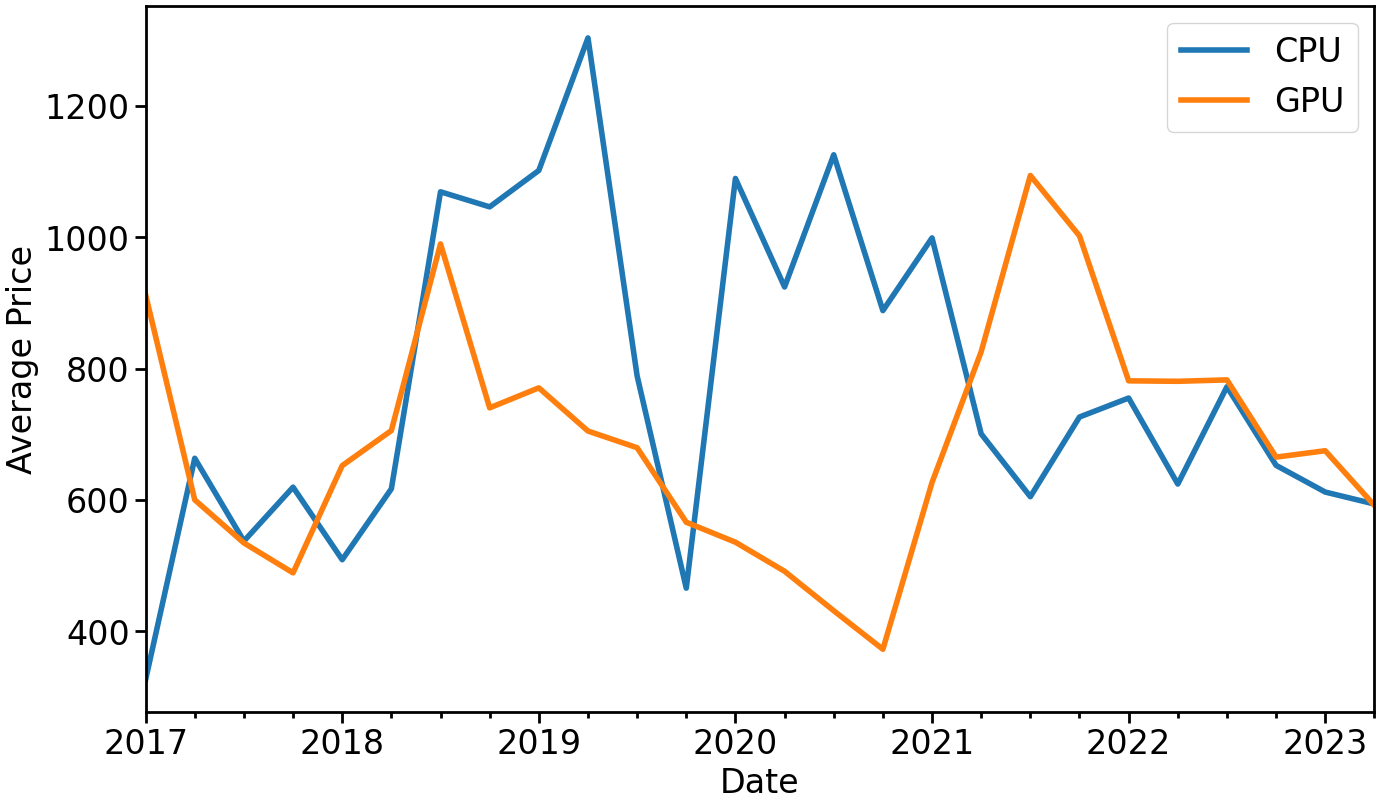
\includegraphics[width=\columnwidth]{avg_price.png}}
	\caption{Inflated average pricing history of CPUs and GPUs}
	\label{fig3}
\end{figure}
First, we will summarize the history of the shortage using the average prices
shown in figure \ref{fig3}. We will start our analysis at Q4 2019 as that is
when the shortage started to take effect \cite{Wikipedia:2023}. As we can see,
CPU and GPU prices
were on the decline prior to the pandemic, sitting at around \$450 and \$550
respectively. But as soon as Q1 2020 hit, CPU price spiked to about \$1050,
more than double its price at the end of 2019! This is due to the drastic
shift to remote working and learning in various countries coupled with the
shutdown of many chip supply chains in favor of practicing social distancing.
This was not the case for GPUs however, presumably because most remote jobs
require CPUs more than GPUs, whose price continued to decline. CPU price
remained stagnate while that of GPU keep decreasing until Q4 2020 when the
China-United States trade war started which caused both prices to increase.
In 2021, as CPU production picked up, its price significantly dropped.
However, GPU prices kept growing due to the upsurge in demands from the
cryptocurrencies mining craze. After which, in Q3 2021, GPU prices started
to drop while CPU prices oscillated around \$700. Today, the average CPU and
GPU prices are around \$600.

Comparing these prices with those from the pre-shortage era (2017 -- 2019), we
can conclude that CPU prices have already recovered from the shortage since
about Q2 2021. On the other hand, although GPU prices have only stabilized
since Q3 2022, they are still on the decline today. Thus, we can conclude that
the processor shortage had already ended in Q3 2022. However, as our historical
analysis on the shortage might suggest, the processor shortage was not caused
by a single advent, but rather a series of events. If this series of events
continues, it is likely that the shortage will reemerge. Ultimately, this
result should be taken with a grain of salt.

\subsubsection{Prediction using polynomial regression}
\begin{figure}[htbp]
	\centerline{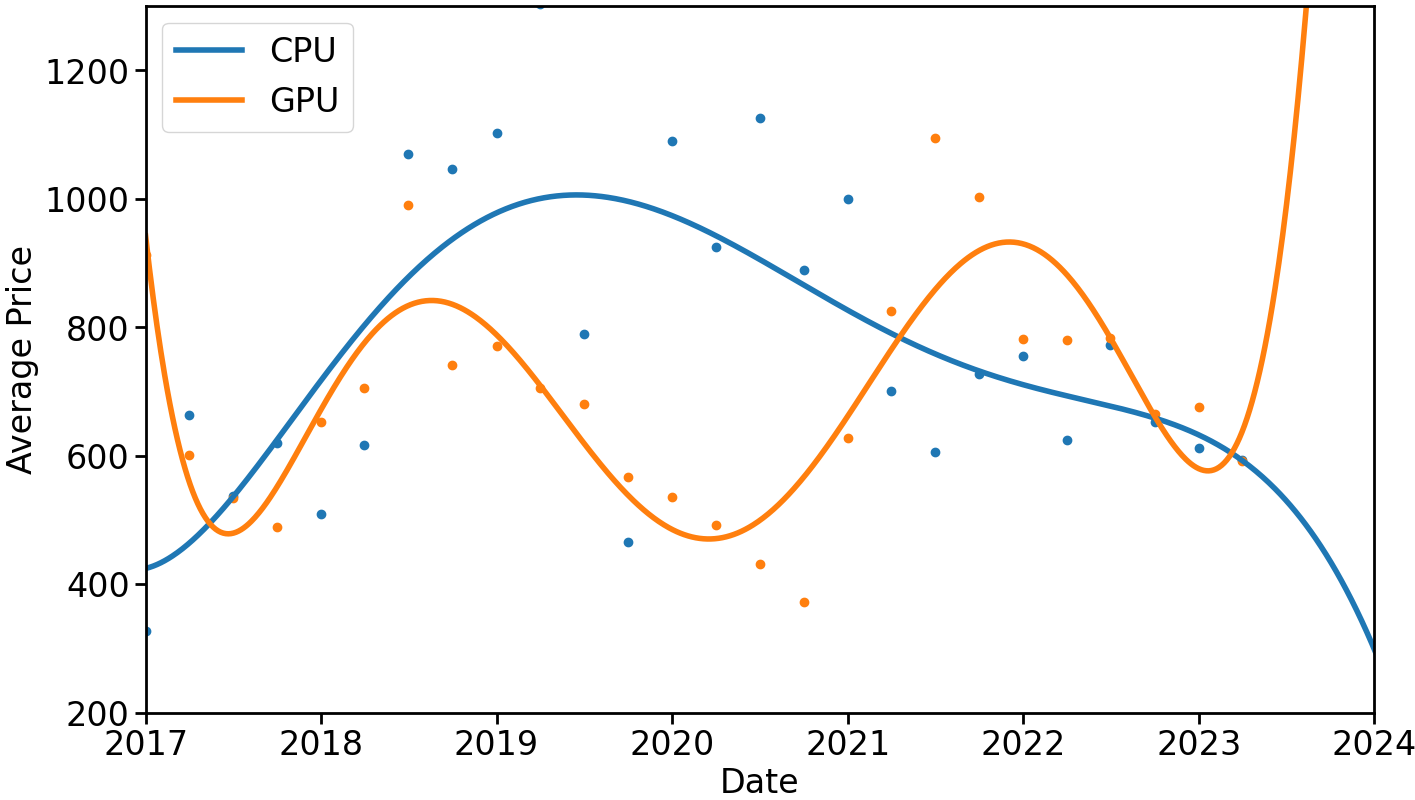
\includegraphics[width=\columnwidth]{avg_price_reg.png}}
	\caption{Average pricing history with polynomial regression curves}
	\label{fig4}
\end{figure}
The polynomial regression curves shown in figure \ref{fig4} are both of degree
6 as that is the optimal degree suggested by NumPy to ensure that we won’t
overfit. The CPU curve, sporting an $R^{2}$ value of $0.49$, suggests that
CPU prices will continue to drop, down to \$300 in 2024. On the other hand,
the GPU curve, with an $R^{2}$ value of $0.74$, forecasts that GPU prices will
skyrocket to unprecedented figures...

Unfortunately, as the pricing history is rather chaotic with no real pattern,
our regression models are unreliable at predicting even the nearest future
regardless of their $R^{2}$ values. Thus, it is evidently better to rely
on our educated guess instead.

\subsubsection{Conclusion}
All in all, we conclude that the shortage had already ended in Q3 2022.
However, there is a slight chance that the shortage will reemerge should
there be another global advent similar to in recent years.

\subsection{What will be the next big thing in the development of
	processors in terms of performance, efficiency, and value?}

\subsubsection{Performance}


\subsubsection{Efficiency}

\subsubsection{Value}

% Todo Revise

\section{Discussion}
% Todo Write and Revise

\section{Conclusion}
% Todo Write and Revise

\section{Acknowledgments}
I would like to express my greatest gratitude to my supervisor,
Doctor Nguyen Ngoc Thao, for not only providing crucial feedback at the start
of the research but also guiding us throughout our endeavor, ultimately shaping
this research up to what it is today.

I am also grateful to my teammates who greatly supported me during
this journey. Without their running me errands and their occasional burst of
good ideas, I would not have been able to finish this research within the
confine of the deadline. Though, I would appreciate it more had they
provided me with more moral support.

Lastly, I would also like to mention some of my classmates whose ideas I
\sout{stole} borrowed for this research.

\bibliographystyle{unsrt}
\bibliography{THUD}

\end{document}